\documentclass[10pt,a4paper]{article}
\usepackage[utf8]{inputenc}
\usepackage[german]{babel}
\usepackage[T1]{fontenc}
\usepackage{fullpage}
\usepackage{amssymb}
\usepackage{listings}
\usepackage{caption}
\usepackage{color}
\usepackage{amsmath}
\usepackage{graphicx}
\usepackage[backend=bibtex]{biblatex}
\usepackage{hyperref}
% Bibliography
\addbibresource{bibliography.bib}
% Code snippet style
% Python colored syntax highlighting
\usepackage{listings}
\usepackage{color}
\usepackage{amsmath}
\definecolor{dark-gray}{RGB}{135,135,135}
\definecolor{light-blue}{RGB}{102,178,255}
\definecolor{light-orchid}{RGB}{210,120,210}
\lstdefinelanguage{python-color}{
 morekeywords={and, as, assert, break, class, continue, def, del, elif, else, except, exec, finally, for, from, global, if, import, in, is, lambda, not, or, pass, print, raise, return, try, while, with, yield, None, True, False, import},
 ndkeywords={self},
 keywordstyle=\color{blue}\bfseries,
 ndkeywordstyle=\color{light-orchid}\bfseries,
 sensitive=false,
 identifierstyle=\color{black},
 basicstyle=\sffamily ,
 morecomment=[l]{\#},
 morecomment=[s]{/*}{*/},
 morecomment=[s]{"""}{"""},
 morecomment=[l][\color{light-blue}]{@},
 morecomment=[s][\color{light-blue}]{"}{"},
 commentstyle=\itshape\color{dark-gray},
 stringstyle=\color{red}\ttfamily,
 tabsize=2,
 columns=fullflexible,
 literate={^}{{$\mspace{-3mu}\hat{\quad}\mspace{-5mu}$}}1
 {<}{$<$}2 
 {>}{$>$}2 
 {<:}{{$<\mspace{-3mu}:$}}2 
 {:>}{{$:\mspace{-3mu}>$}}2
 {+}{$+$ }2 
 {++}{{$+\mspace{-8mu}+$ }}2
 {\~}{{$\mspace{-3mu}\tilde{\quad}\mspace{-3mu}$}}1
 {\~}{$\sim$}1
 {__}{\underline{\hspace{0.5cm}}}1
 {*}{${}^{\ast}$}1 
 {.}{$\mspace{1mu}.\mspace{1mu}$}1
}
\lstset{language=python-color}
\lstset{framexleftmargin=5pt, framextopmargin=5pt, framexbottommargin=5pt, frame=tb, framerule=0pt}
\definecolor{grey}{rgb}{0.9,0.9,0.9}
%\newcounter{nalg}[section] % defines algorithm counter for chapter-level
%\renewcommand{\thenalg}{\thechapter .\arabic{nalg}} %defines appearance of the algorithm counter
%\DeclareCaptionLabelFormat{algocaption}{Algorithm \thenalg} % defines a new caption label as Algorithm x.y

\lstnewenvironment{algorithm}[1][] %defines the algorithm listing environment
{   
    %\refstepcounter{nalg} %increments algorithm number
    %\captionsetup{labelformat=algocaption,labelsep=colon} %defines the caption setup for: it ises label format as the declared caption label above and makes label and caption text to be separated by a ':'
    \lstset{ %this is the stype
        mathescape=true,
        keywordstyle=\color{black}\bfseries\em,
        keywords={,input, output, return, datatype, function, in, if, else, foreach, while, begin, end, for, endfor, from, to, do, loop, print, }, %add the keywords you want, or load a language as Rubens explains in his comment above.        
        #1 % this is to add specific settings to an usage of this environment (for instnce, the caption and referable label)
    }
}
{}

\setlength{\parindent}{0pt}
\setlength{\columnsep}{0.5cm}

\title{Teil II:\\Ausarbeitung zum WEP-Protokoll}
\author{Lukas Jung, Oliver Sänger, Tobias Zeimetz, Marc Narres-Schulz}

\begin{document}
\maketitle
\tableofcontents
\newpage

\section{Einführung}
Bei der vorliegenden Arbeit handelt es sich um ein Protokoll über eine Teilaufgabe im \glqq Hackerpraktikum\grqq . Die erste Aufgabe bestand darin, sich in WEP und RC4 einzuarbeiten. Die relevante Literatur für das Verständnis von WEP und RC4 waren folgende Artikel: \glqq Attacks on the RC4 stream cipher\grqq \cite{Kle08}, \glqq Breaking 104 bit WEP in less than 60 seconds\grqq \cite{TWP07}\ und \glqq Intercepting Mobile Communications: The Insecurity of 802.11\grqq \cite{BGW01}.\\
Anschließend sollte eine Testumgebung und der Angriff nach Klein umgesetzt werden. Diese bestand aus einer Simulation der RC4-Stromchiffre und lieferte  Paare aus Initialisierungsvektor (IV) und Stromchiffre. Das Ziel des Angriffs nach Klein war es, auf dieser Grundlage den Hauptschlüssel zu berechnen und somit die Verschlüsselung zu brechen.
Die letzte Teilaufgabe bestand darin, den Hauptschlüssel eines Routers zu berechnen, der mit WEP konfiguriert wurde. Dazu wurden Paare aus IV und Schlüsselstrom benötigt. Diese lassen sich mittels \glqq ARP-Reinjection\grqq\ generieren. Mit den erzeugten Daten konnten wir den Angriff von Klein durchführen. Als Ergebnis erhielten wir den Hauptschlüssel der Verschlüsselung. Zusätzlich haben wir die Verbesserungen aus dem Paper \glqq Breaking 104 bit WEP in less than 60 seconds\grqq \cite{TWP07}\ umgesetzt und die beiden Angriffe miteinander verglichen.\\
Das Protokoll besteht aus drei Teilen. Im ersten Abschnitt werden die Grundlagen der Verschlüsselung erläutert. Dort wird die Funktionsweise der RC4-Stromchiffre, die des WEP-Protokolls und damit zusammenhängende Begrifflichkeiten dargestellt. Anschließend wird im Detail auf den Angriff von Klein und dessen Verbesserung eingegangen. Abschließend haben wir die Performance und die Erfolgsquote beider Versionen verglichen. 
\section{Grundlagen}
Es folgt eine Einleitung in die Funktionsweise der RC4-Stromchiffre und des WEP-Protokolls.
\subsection{RC4-Stromchiffre}
Der Algorithmus zu RC4 wurde 1987 von Ron Rivest entwickelt und besteht aus zwei Teilen. Der erste Teil ist das \glqq key scheduling\grqq\ und der zweite Teil ist eine \glqq pseudo random generation\grqq . Der RC4-Algorithmus erhält als Eingabe einen Schlüssel. Im ersten Schritt erzeugt dieser in der \glqq key scheduling\grqq -Phase aus dem Schlüssel eine Permutationstabelle (S-Box). Nachfolgend wird die S-Box in der \glqq pseudo random generation\grqq\ zur Erzeugung einer Pseudozufallssequenz genutzt.\\
Die \glqq key scheduling\grqq -Phase mit Schlüssel $K$ als Eingabe läuft wie folgt ab:
\begin{center}
\hspace{5pt}
\begin{minipage}[t]{.35\textwidth}
\begin{algorithm}
{initialization}
for i from 0 to n-1 do
    S[i] := i
end for
j := 0
{generate a random permutation}
for i from 0 to n-1 do
    j := (j+S[i]+K[i mod l]) mod n
    Swap S[i] and S[j]
end for
\end{algorithm}
\end{minipage}\hspace{0.4cm}
\begin{minipage}[t]{.60\textwidth}
  \begin{lstlisting}
def keyScheduling(sessionKey=bytearray(), n=256):
	# initialization
	sBox = []
	for i in range(n):
   		sBox.append(i)
   		sBox = bytearray(sBox)

   	i,j = 0,0
   	# generate a random permutation
   	for i in range(n):
     	j = (j + sBox[i] + sessionKey[i % len(sessionKey)]) % n
    	sBox[i], sBox[j] = sBox[j], sBox[i]

	return sBox
\end{lstlisting}
\end{minipage}
\end{center}

Bei der \glqq key scheduling\grqq -Phase wird die S-Box initialisiert und mit den Werten aus 0 bis $n-1$ aufsteigend gefüllt. Die S-Box wird aus dem  Schlüssel berechnet und später zur Berechnung der Stromchiffre verwendet. In jedem Schritt der \textit{for}-Schleife werden zwei Einträge der S-Box vertauscht um eine pseudozufällige Permutation zu erzeugen. Diese lässt sich von einer echt-zufälligen Permutation unterscheiden \ref{ssec:schwäche}.\\
In der zweiten Phase des RC4-Algorithmus wird eine Zufallsfolge, im Folgenden auch Stromchiffre genannt, erstellt:
\begin{center}
\hspace{5pt}
\begin{minipage}[t]{.35\textwidth}
\begin{algorithm}
{initialization}
i := 0
j := 0
{generate pseudo random sequence}
loop
    i := (i + 1) mod n
    j := (j + S[i]) mod n
    Swap S[i] and S[j]
    k := (S[i] + S[j]) mod n
    print S[k]
end loop
\end{algorithm}
\end{minipage}\hspace{0.4cm}
\begin{minipage}[t]{.60\textwidth}
\begin{lstlisting}
def pseudoRandomGenerator(sBox=bytearray(),n=256):
   	# initialization
	i,j = 0,0

	# generate pseudo random sequence
	while True:
   		i = (i + 1) % n
   		j = (j + sBox[i]) % n
   		sBox[i], sBox[j] = sBox[j], sBox[i]
   		k = (sBox[i] + sBox[j]) % n

   		yield bytes([sBox[k]])
\end{lstlisting}
\end{minipage}
\end{center}
Hierbei handelt es sich um den Hauptteil des RC4-Algorithmus. Der pseudozufalls-Generator erhält die S-Box aus der \glqq key scheduling\grqq -Phase als Parameter. Darauf wird ein Index $j$ mit Hilfe der zufällig permutierten S-Box gewählt und zwei Einträge ($sBox[i]$ und $sBox[j]$) vertauscht. Der nächste Schritt besteht darin einen Index $k$ zu ermitteln, welcher aus den addierten Werten aus der S-Box bestehen. Durch den anschließenden Modulo-Operator wird sichergestellt, dass es sich um Werte aus dem Zahlenraum $\mathbb{Z}_n$ handelt. Der pseudozufalls-Generator erstellt somit in jedem Schritt ein Byte, mit einem Wert zwischen im genannten Zahlenraum ($0$ bis $n-1$) als Ausgabe.
\subsubsection{Schwächen in RC4}\label{ssec:schwäche} 
Die von RC4 erzeugte Pseudozufallssequenz (PZS) unterscheidet sich in einigen Punkten von einer echten Zufallsfolge. Die Summe der letzten Bits in Schritt t und t+2 korreliert gegen 1.
J.Dj. Golic kam zu dem Schluss, dass ${2}^{40}$ Bytes von der RC4-PZS unterscheidbar sind zu einer echten Zufallssequenz.\\
Weitere Untersuchungen von S.R. Fluhrer und D.A. McGrew haben bewiesen, das die Wahrscheinlichkeit von zwei aufeinander folgenden Bytes sich signifikant von einer Zufallsfolge unterscheiden. Im Idealfall besteht ein Schlüssel aus n unabhängig, identischen und gleichverteilten Elementen aus $\mathbb{Z}_n$ und generiert $n^n$ gleichwahrscheinliche Schlüssel. Jedoch ist $n!$ kein Teiler von $n^n$. Daher muss sich die Verteilung der initialen Permutation von einer Gleichverteilung unterscheiden. (Siehe Studie von I.Mironov)
Für das weitere Vorgehen ist jedoch folgende Schwachstelle wichtig:\\
Das erste Byte der PZS wird nicht zufällig gewählt. Der Angriff von S. Fluhrer, I. Martin und A. Shamir \cite{FMS01} nimmt an, dass der IV vor dem Schlüssel steht und die ersten zwei Bytes die Form $(b,n-1)$ haben, wobei $b$ das Byte des Schlüssels ist, welches rekonstruiert werden soll. Wenn ein Angreifer keine Chance hat den IV zu beeinflussen, muss er warten, bis dieser die gewünschte Form annimmt. Die ist in durchschnittlich einer aus $n^2$ Sitzungen der Fall. Die Autoren zeigen, dass dieser Angriff auf WEP angewendet werden kann.
\subsection{WEP}\label{ssec:wep}
Wired Equivalent Privacy (WEP) ist ein Standard aus dem Jahr 1999 für WLANs. Das Protokoll wurde dazu verwendet um die Vertraulichkeit und Integrität einer Nachricht sicherzustellen. Für die Verschlüsselung waren zwei Modi relevant. Die Länge des Schlüssels $k$ und des Initialisierungsvektors $v$ sind dabei abhängig vom gewählten Modus.
\begin{itemize}
\item 64-Bit-Verschlüsselung: IV-Länge 24 Bit, Schlüssellänge 40 Bit
\item 128-Bit-Verschlüsselung: IV-Länge 24 Bit, Schlüssellänge 104 Bit
\end{itemize}
Die Verschlüsselung eines Nachrichtenpaketes $M$ unter WEP läuft wie folgt ab:\vspace{0.5em}
\begin{center}
$C = (M || c(M)) \oplus RC4(v || k)$
\end{center}
Zuerst wird über eine Nachricht $M$ eine Prüfsumme $c(M)$ gebildet. Anschließend wird die Nachricht $M$ mit $c(M)$ konkateniert in der Form $(M || c(M))$. Der nächste Schritt besteht darin den RC4-Algorithmus aufzurufen und so viele zufällige Bytes zu produzieren wie der Term $(M || c(M))$ besitzt. Bei den Variablen die der RC4-Funktion übergeben werden, handelt es sich zum einen um einen zufällig gewählten Initialisierungsvektor $v$ und den Schlüssel $k$.\\
Der letzte Schritt besteht darin die zufällige Bytefolge $RC4(v || k)$ und den Term $(M || c(M)$ mittels XOR zu verrechnen. Dadurch entsteht eine Vernamchiffre $C$ die nur bei Kenntnis von $v$ und $k$ (und letztendlich $RC4(v || k)$) entschlüsselt werden kann. Die Konkatenation von IV und Schlüssel bilden den \glqq session key\grqq .\\
Über das Netzwerk werden durch den Router Nachrichten verschickt, welche die Form $v || C$ besitzen. Der Initialisierungsvektor wird dabei vorne and die Vernamchiffre konkateniert. Da die Länge des Initialisierungsvektors $v$ bekannt ist, kann der Empfänger der Nachrichten diesen \glqq abschneiden\grqq\ und durch Kenntnis des Schlüssels $k$ die Stromchiffre $RC4(v || k)$ erzeugen. Abschließend kann durch $RC4(v || k) \oplus C$ die Chiffre $C$ entschlüsselt werden.\\
Durch die Prüfsumme $c(M)$ ist der Empfänger in der Lage, die Integrität der eigentlichen Nachricht $M$ zu gewährleisten. 
\section{Umsetzung}
In diesem Abschnitt werden die verschiedenen Angriffe die wir in den Aufgaben 2 bis 4 durchführt haben genauer dargelegt. Der erste Abschnitt befasst sich mit der Anwendung des Klein Angriffs auf den RC4-Algorithmus in einer \glqq simulierten Umgebung\grqq . Anschließend wird der Angriff in realer Umgebung ausgeführt. In diesem Zusammenhang wird darauf eingegangen wie man das Auftreten von ARP-Paketen mit Hilfe von \glqq ARP-Reinjection\grqq\ erhöht. Weiter werden aus den gewonnenen Paketen Paare von IV und Schlüsselstrom extrahiert und der Angriff von Klein wird auf diese Daten angewendet. Abschließend wird erläutert wie man den Angriff deutlich effizienter gestalten kann. Im Folgenden wird größtenteils die Notation aus dem Paper \cite[Kapitel 3.1]{TWP07} verwendet.
\subsection{Angriff}\label{ssec:klein}
Der Angriff von Klein nutzt nun die oben beschriebene Schwäche von RC4 aus. Wir betrachten die Permutation in der \glqq key scheduling\grqq -Phase.\\
Hier sieht man leicht, nach dem ersten Schritt gilt für Bytes des Schlüssels K und Werte der S-Box S:
\begin{center}
$ j = 0+0+K[0] = K[0] $
\\\vspace{0.5em}
$\Rightarrow S[0] \textit{ wird vertauscht mit }  S[K[0]] $\\
\end{center}
So lässt sich die zweite Runde (mit Wahrscheinlichkeit $1 - (1/n)$) ebenfalls rekonstruieren:
\begin{center}
$ j = K[0] + 1 + K[1]$
\\\vspace{0.5em}
$\Rightarrow S[1] \textit{ wird vertauscht mit } S[ K[0] + 1 + K[1] ] $
\end{center}
( $K[0] + 1 + K[1]$ ) wird im Weiteren mit  $t$ bezeichnet. Wir wissen nun, dass für ein festes $K[0]$ der Wert $t$ und $S[1]$ sich aus $K[1]$ berechnen lassen. In den weiteren Schritten der \glqq key scheduling\grqq -Phase wird $S[1]$ nicht mehr geändert, sofern $j$ nie den Wert 1 annimmt.
Die Wahrscheinlichkeit, dass dies in einem Schritt dennoch passiert liegt bei $1 - \frac{1}{n}$ falls der \glqq session key\grqq\ die Länge n hat.
Sind alle Schlüsselbytes von einander unabhängig, folgt $S[1]$ wird mit der Wahrscheinlichkeit $(1-\frac{1}{n})^{n-2} \approx \frac{1}{e}$ nicht verändert.\\
Nun wissen wir Folgendes:\\
Der Wert von $S[1]$ ist zu Beginn des RC4-PZG $t$. Wobei $t$ mit Wahrscheinlichkeit $(1/e)$ nur von $K[0]$ und $K[1]$ abhängt. Somit kann das in der Arbeit von Klein hergeleitete Theorem 1 \cite{Kle08} benutzt werden um $t$ aus der beobachteten RC4-PZS zu erhalten.\\
Dazu schauen wir uns die Generierung des ersten Pseudozufall-Bytes (PZB) an:\\
Zuerst wird $i$ auf $1$ gesetzt. Daher werden $S[1]$ und $S[j]$ getauscht. Nun enthält $S[j]$ den interessanten Wert t und nach Theorem 1 folgt: 
\begin{center}
$S[j] = 1 - S[k]\ mod\ n$ mit Wahrscheinlichkeit $\frac{2}{n}$
\end{center}
Nutzt man diese Aussagen, kommt man zu folgender Approximation für t:
\begin{center}
$Prob( t = 1 - S[k] mod n) \approx \dfrac{1}{e} * \dfrac{2}{n} + ( 1- \dfrac{1}{e}) * \dfrac{n-2}{n(n-1)} \approx 1.36/n$
\end{center}
Unser Angriff hat nun folgende Form:\\
Für verschiedene IVs (n-Stück) können wir die ersten Bytes $x_i$ mit $1 <= i <= n$ beobachten und $t_i = 1 - x_i$ ausrechnen. Wie Wahrscheinlichkeit, das $t_i$ den richtigen Wert annimmt liegt bei $1.36/n$ alle anderen Werte haben eine Wahrscheinlichkeit von unter $1/n$. Wenn die Anzahl der Sessions groß ist, kann man das Schlüsselbyte an der ersten Stelle mit hoher Wahrscheinlichkeit bestimmen.\\
Die folgenden Schlüsselbytes können nun iterativ berechnet werden. Kennt man die Schlüsselbytes bis zur Stelle $i\ ( mit\  i < |Key|)$, so kennt man auch den internen Zustand der S-Box bis zu dieser Stelle und den Index $j$ im Schritt $i - 1$ des RC4-\glqq key scheduling\grqq -Algorithmus. \\
Die weiteren Schlüsselbytes sind folglich berechenbar durch:
\begin{center}
$\mathcal{F}_i(K[0], .\ .\ .\ ,K[i-1],X[i-1]) = \begin{cases} K[i], mit \ Prob \approx 1.36/e \\ \alpha \neq K[i], mit \ Prob < 1/n \\\end{cases}$
\\\vspace{1em}
$\mathcal{F}_i(K[0], .\ .\ .\ ,K[i-1],X[i-1]) = S^{-1}_{i-1}[i-X[i-1]] - (j_{i-1}+S_{i-1}[i]) \ mod \ n$
\end{center}
\subsubsection{Anwendung auf WEP}
Wir haben den Angriff von Klein erfolgreich auf WEP40 und WEP104 angewand.
In WEP-Protokoll haben die Pakete die folgende Form: $IV || Chiffreschlüsselstrom $. Bei beiden Protokollen haben die Initialisierungsvektor eine Länge von 24 Bit (= 3 Byte). Aus diesem Grunde ist es nicht nötig die ersten 3 Bytes des Hauptschlüssels mit der Methode von Klein zu berechnen. Es kann direkt mit der iterativen Berechnung der Schlüsselbytes begonnen werden. Mithilfe von \glqq ARP-Reinjection\grqq\ haben wir circa 500.000 IV und Chiffreschlüsselstrom generiert. Die ersten 16 Bytes eines ARP-Paketes sind immer gleich. Da der erzeugte Schlüsselstrom mit dem Klartext lediglich über eine XOR-Operation zur Stromchiffre verknüpft wird, erhalten wir durch die erneute Anwendung der XOR-Operation den erzeugten Schlüsselstrom. Hat man nun genug Paare gesammelt, lässt sich mit Hilfe des zuvor beschriebenen Angriffes der Hauptschlüssel berechnen. Bereits nach 35.000 untersuchten ARP-Paketen konnten wir zuverlässig den Hauptschlüssel für WEP40 errechnen. Für WEP104 benötigten wir für eine zuverlässige Aussage ca. 45.000 Pakete. Die Laufzeit betrug hierbei im Mittel 5 Sekunden für WEP40 und 60 Sekunden für WEP104. Beide Werte berücksichtigen nicht das Sammeln von ARP-Paketen. Dies dauert in der Regel 3 bis 5 Minuten. Im Abschnitt \ref{ssec:vergleich} werden wir noch genauer auf die Laufzeit eingehen.
\subsubsection{Simulation}
Wie bereits erwähnt, bestand ein Teil der Aufgaben darin, den Angriff von Klein auf selbst generierte Paare von IV und Stromchiffren anzuwenden. Dazu wurde ein Package \glqq RC4\grqq\ erstellt, indem die Methoden für die \glqq key scheduling\grqq -Phase und den \glqq pseudo random generator\grqq enthalten waren. Außerdem beinhaltet das Package eine Methode mit dem Namen $fixed\_rc4$ die zur Ausgabe eines RC4-Stromchiffre fester Länge genutzt wird.
\begin{lstlisting}
		def fixed_rc4(key, cipher_length, n):
    		# Initial permutation
    		s_box = key_scheduling(key, n=n)
    		cipher = bytearray()
    		# Extract cipher_length stream key bytes
    		for k in pseudo_random_generator(s_box):
        		cipher += k
        		if len(cipher) >= cipher_length:
            		break
    		return cipher
\end{lstlisting}
Die Methode ruft den \glqq key scheduling\grqq -Algorithmus auf und erzeugt somit eine permutierte S-Box. Neben dem Zahlenraum $\mathbb{Z}_n$ der mittels $n$ übergeben wird, wird auch der Schlüssel $k$ und die Länge der Stromchiffre übergeben. Dadurch werden in der For-Schleife genau so viele zufällige Bytes generiert wie gefordert. Wurde die maximale Anzahl an zufälligen Bytes generiert bricht der Algorithmus ab und gib die pseudozufällige Bytefolge aus.
% Paar generierung erklären
% Method for generation of (iv, main key and stream key) pairs as required by Exercise 2.2 (Modes: 64-bit WEP(WEP-40): 40 bit key, 24-bit iv, 128-bit WEP(WEP-104): 104 bit key, 26-bit iv )
\begin{lstlisting}
def iv_and_stream_cipher_generator(n, rounds, iv_length, key_length, tuple_amount):
    # Generate random key
    main_key = bytearray(os.urandom(key_length))

    iv_stream_set = []
    for i in range(tuple_amount):
        # Generate random iv
        iv = bytearray(os.urandom(iv_length))
        stream_cipher = fixed_rc4(iv, main_key, cipher_length=rounds * n, n=n)
        iv_stream_set.append((iv, stream_cipher))
    return iv_stream_set, main_key
\end{lstlisting}
Diese Funktion erzeugt Paare aus IV und Stromchiffre für einen festen Schlüssel, wie sie in der WEP Verschlüsselung Verwendung finden. Zunächst wird ein Schlüssel und ein IV, deren Länge durch den verwendeten Modus \ref{ssec:wep} bestimmt werden, zufällig gewählt. Dann werden mit dem zuvor beschriebenen Algorithmus, IV und Schlüssel eine feste Anzahl dieser Paare generiert, wobei der IV nach jeder Iteration erneut zufällig gewählt wird. Die Menge an Paaren werden zusammen mit dem Schlüssel zurückgegeben. Der Schlüssel dient der Verifikation eines Angriffs.
\subsubsection{Angriff}
\paragraph{ARP-Pakete generieren}
Das Internet Protocol (IP) ist das am weitesten verbreitete Netzwerkprotokoll. Für unseren Angriff gehen wir davon aus, dass IPv4 im anzugreifenden WLAN verwendet wird. Wenn Host A ein Paket an Host B senden möchte, benötigt A die physikalische Adresse des Hosts B oder des Gateways, durch das B erreicht werden kann. Zum Auflösen der IP-Adressen wird das Address Resolution Protokoll (ARP) verwendet. Dies funktioniert wie folgt: Host A sendet eine ARP-Anfrage an die Broadcast-Adresse. Diese Anforderung gibt an, dass A nach der physikalische Adresse von Host B sucht. Host B antwortet mit einer ARP-Antwort mit seiner eigenen physikalische Adresse an Host A. ARP ist ein Link-Layer-Protokoll, daher ist es in der Regel nicht durch Paket-Filter oder Senderate beschränkt. ARP-Anfragen und ARP-Antworten sind von fester Größe. Da die Größe eines Pakets nicht durch WEP maskiert wird, können sie in der Regel leicht von anderen unterschieden werden. Die ersten 16 Bytes eines Klartextes eines ARP-Pakets bestehen aus einem 8 Byte langen 802.11 Logical Link Control (LLC)-Header gefolgt von den ersten 8 Bytes der ARP-Paket selbst. Der LLC-Header ist für jedes ARP-Paket festgelegt:\\
\begin{center}
	AA AA 03 00 00 00 08 06\\
\end{center}
Die ersten 8 Bytes einer ARP-Anfrage sind ebenfalls fixiert. Ihr Wert ist:\\
\begin{center}
	00 01 08 00 06 04 00 01\\
\end{center}
Bei einer ARP-Antwort ändert sich das letzte Byte zu 02. Eine ARP-Anfrage wird immer an die Broadcast-Adresse gesendet, während eine ARP-Antwort an einen Unicast gesendet wird. Da die physikalischen Adressen nicht durch WEP verschlüsselt werden, ist es einfach zwischen einer verschlüsselten ARP-Anfrage und Antwort zu unterscheiden. Durch das Verrechnen eines erfassten ARP-Pakets mit diesen festen Mustern können wir die ersten 16 Byte des Schlüsselstroms extrahieren. Der entsprechende IV wird im Klartext übertragen. Um die Wiederherstellung von Schlüsselstrom zu beschleunigen, ist es möglich, einen erfassten ARP erneut zu injizieren, was im Netzwerk, die eine weitere Antwort mit neuem IV auslöst. Wenn der Initiator und das Ziel der ursprünglichen Anfrage beide WLAN-Stationen sind, werden drei neue Pakete generieren, da die Übertragung vom Access Point weitergeleitet wird. Das Sammeln von genügend Paketen dauert nur wenige Minuten. Um Pakete zu erzeugen und zu speichern wurden \glqq aireplay-ng\grqq\ und \glqq airodump-ng\grqq\ verwendet.
\paragraph{Angriff nach Klein}\label{p:klein_attack}
Die Theorie zum Angriff von Klein wird auf Seite \pageref{ssec:klein} beschrieben. Dieser wurde von uns in Python umgesetzt und in einer Testumgebung erfolgreich getestet. 
Mittels ARP-Reinjection haben wir über 500.000 ARP-Pakete gesammelt. Wie im vorherigen Kapitel beschrieben, sind waren wir somit in der Lage den Schlüsselstrom zu rekonstruieren. 
Im Anschluss wurden die Schwächen von RC4 ausgenutzt um auf den Schlüssel zu kommen. Der in Kapitel \ref{ssec:klein} beschriebene Ablauf wurde hierzu nachvollzogen und  in Python simuliert. Wir werden im Folgenden nicht den Programmcode im Detail erklären, sondern beschränken uns auf die wichtigsten Schritte.\\
Wir kennen die drei ersten Bytes des \glqq session key\grqq\ ,da der IV jedem Paket vorsteht. Somit kann der innere Zustand der S-Box bis zu dieser Stelle simuliert werden. Nun kennen wir die S-Box sowie die Indizes i und j zu diesem Zeitpunkt. Wir können nun mithilfe der Formel aus Kapitel \ref{ssec:klein} für alle gesammelten Pakete einen Kandidaten für die nächste Stelle bestimmen. Der Wert, welcher für diese Stelle am häufigsten auftritt, ist mit hoher Wahrscheinlichkeit (siehe \ref{ssec:klein}) das gesuchte Schlüsselbyte. Dieses Vorgehen wird iterativ angewandt bis ein möglicher Schlüssel feststeht.
Um diesen Schlüssel zu verifizieren, wird ein gesammeltes (IV,Stromchiffre)-Paar mit dem Schlüssel verschlüsselt und auf Gleichheit geprüft. Ist dies der Fall, hat man den Schlüssel gefunden.\\
Schlägt dieser Test fehl, muss man den Angriff mit mehr Paketen wiederholen. Ab 80.000 Paketen lieferte der Angriff zuverlässig (mit einer Wahrscheinlichkeit von über 90\%) den Schlüssel.
\subsubsection{Verbesserung des Angriffs}
Folgende Verbesserungen gehen aus dem Paper \glqq Breaking 104 bit WEP in less than 60 seconds\grqq \cite{TWP07}\ hervor.
In Klein's Angriff werden die Schlüsselbytes iterativ berechnet, das bedeutet die Berechnung des Bytes $K[i]$ ist abhängig von seinen Vorgängern $K[0] \cdot\ \cdot\ \cdot\ K[i-1]$. Dies ist nicht optimal, denn die Paare aus Initialisierungsvektor und Stromchiffre müssen gespeichert werden und das Korrigieren potenzieller Fehler ist teuer \cite[Kapitel 4]{TWP07}.\\
Die von Tews et al. vorgestellte Methode verwendet eine parallelisierte Berechnung von sogenannten \glqq votes\grqq\ für Schlüsselbytes und einem anschließenden \glqq key ranking\grqq . Diese ist wesentlich schneller und fehlertoleranter, da sie nicht auf den Werten vorangegangener Schlüsselbytes beruht.\\
Ihr Ansatz macht Annahmen über den Zustand der S-Box \cite[Kapitel 4, (4)-(5)]{TWP07} und basiert auf einer Umformung des Angriffs von Klein. Dieser erlaubt die Berechnung von $K[i]$ ohne zusätzliches Wissen über die Werte $K[0] \cdot\ \cdot\ \cdot\ K[i-1]$. Die Annahme führt jedoch dazu, dass besonders geformte Schlüsselbytes, sogenannte \glqq strong key bytes\grqq\ im Schlüssel auftreten können. Handelt es sich um ein starkes Schlüsselbyte, muss dieses erkannt und korrigiert werden. Sollte der Schlüssel aus vielen starken Schlüsselbytes bestehen (bei WEP104 z.B. 12 Bytes) wird die Methode mit Schlüsselranking ineffizient und muss ohne Schlüsselranking ausgeführt werden.
\paragraph{Parallelisierte Berechnung}\label{ssec:p2}
Aus den von Klein postulierten Formeln zur iterativen Berechnung von Schlüsselbytes \ref{ssec:klein}, wird durch eine Reihe von Umformungen \cite[Kapitel 4, Formeln (3)-(5)]{TWP07} die folgende Formel gewonnen. Rk bezeichne den Schlüssel aus IV || Rk.
\begin{center}
\[\sigma_i \approx_n S_3^{-1} [(3 + i) - X[2 + i]] - \left(j_3 + \sum_{l=3}^{i+3} S_3[l]\right)\]
\\\vspace{0.2em}
\[\sigma_i = \sum_{l=3}^{3+i} K[l] = \sum_{l=0}^{i} Rk[l]\]
\end{center}
\vspace{1em}
Diese Umformung basiert nur noch auf den folgenden Angaben:\\
\begin{itemize}
\item $S_3$ und $S_3^{-1}$ (Die normale und invertierte S-Box, permutiert bis zur dritten Stelle mit Hilfe der Schlüsselbytes K[0] bis K[2] bzw. dem IV[0] bis IV[2])
\item X (die Stromchiffre)
\item Indizes i (Position des zu berechnenden Schlüsselbytes) und j (Laufindex aus der Permutation der S-Box)
\end{itemize}
\vspace{0.5em}
Die Wahrscheinlichkeit, dass $\sigma_i$ mit dem berechneten Wert übereinstimmt und das richtige Schlüsselbyte liefert liegt bei 0.5342\% \cite[Kapitel 4, Formel (6)]{TWP07}.\\
Die Formel wird dazu verwendet um \glqq votes\grqq\ für alle Positionen im Schlüssel zu errechnen. Können genügend \glqq votes\grqq\ gesammelt werden, d.h. es stehen genug Paare aus IV und Stromchiffre zur Verfügung, ergibt sich ein Kandidat für den Schlüssel indem man die am häufigsten auftretenden \glqq votes\grqq\ wie folgt auswertet:
\begin{center}
$Rk[i] = \begin{cases}\hspace{0.3em} \sigma_0 \hspace{3.5em}, f\ddot{u}r\ i=0 \\ \hspace{0.3em}\sigma_i - \sigma_{i-1}\hspace{0.5em}, sonst \\\end{cases}$
\end{center}
Die Differenz muss gebildet werden, da die umgeformte Gleichung \ref{ssec:p2} eine Schätzung für die Summe der Schlüsselbytes bis zur Position i ergibt.\\
Bei wenigen Paaren aus IV und Stromchiffre ist der richtige Wert für $\sigma_i$ nicht immer der am häufigsten auftretende Wert unter den \glqq votes\grqq , ist aber meist unter den populärsten Einträgen zu finden. Dies erfordert ein Verfahren zur Kombination von möglichen Schlüsseln aus der zuvor gewonnenen Abbildung von Schlüsselpositionen zu \glqq votes\grqq .
\paragraph{Schlüsselranking}
Das \glqq key ranking\grqq\ verwendet eine Abbildung von Schlüsselbytes K[i] zu Mengen von Schlüsselbytes M[i]. Aus dieser Abbildung werden mögliche Schlüssel kombiniert und an eine Testfunktion weitergegeben. Diese validiert die Korrektheit des möglichen Schlüssels, indem sie RC4 mit IV und dem Kandidatenschlüssel ausführt und die Ausgabe mit der Stromchiffre vergleicht.
\vspace{0.5em}
\\Die Menge V bezeichne eine Abbildung von Schlüsselpositionen auf Mengen von Tupeln aus \glqq vote\grqq\ und Prozent ihres Auftretens (v, p). Sei T eine Menge von Tupeln (v, p), dann sei
\[ \max(T) := v,\ mit\ (v, p) \in T \wedge p = \max (\{p | (v,p) \in T \}) \]
Die Abbildung wird einmal mit dem populärste Schlüssel initialisiert.\\
\begin{center}
$ M[i] \leftarrow \sigma_i\ ,mit\ \sigma_i = max(V[i])$
\end{center}
In jedem weiteren Schritt wird einer der Mengen M[i] ein Byte hinzugefügt, welches den geringsten Abstand zum am häufigsten gewählten Byte in der jeweiligen Menge besitzt.
\begin{center}
\[ \sigma_i = \max_{1 \leq i \leq |K|} (\{v | (v,p) \in V[i] \wedge v \notin M[i]\}) \]
\\\vspace{0.8em}
$ M[i] \leftarrow M[i] \cup \sigma_i$
\end{center}
Nach jedem Hinzufügen wird die Testfunktion mit allen kombinierbaren Schlüsseln, jedoch ohne bereits zuvor getestete Kandidaten, ausgeführt. 
\paragraph{Starke Schlüsselbytes}
Die Umformungen aus \ref{ssec:p2} wurden unter der Annahme getätigt, dass $S_3$ eine Schätzung für $S_{3+i}$ sei. Dies ist für eine bestimmte Menge der möglichen Schlüssel nicht der Fall. Enthält ein Schlüssel ein Byte für das diese Annahme nicht gilt so handelt es sich um ein \glqq strong key byte\grqq\ und bei einem Schlüssel, der mindesten eines dieser Bytes enthält, um einen \glqq strong key\grqq .\\
Genauer betrachtet passiert dies während der Permutation der S-Box. Der Wert für $j_{i+3}$ wird mit j nach Schritt 3 und vor Schritt i+3 getauscht. Daraus resultiert der Tausch von S[$j_{i+3}$] mit einem unbekannten Wert, der abhängig von IV und vorigen Schlüsselbytes ist. Dieser Wert wird in Schritt i+3 mit S[i] getauscht, anstatt des erwarteten S[$j_{i+3}$]. Eine Formel um festzustellen ob ein gegebener Schlüssel ein \glqq strong key byte\grqq\ enthält findet man im Paper \cite[Kapitel 4, Kapitel 6.2, Formel (9)]{TWP07}.\\
Um starke Schlüssel zu erkennen ohne, dass man den Zugriff zu dem Schlüssel selber hat muss man die Häufigkeitsverteilung der erhaltenen \glqq votes\grqq\ betrachten. Tritt in der Verteilung der \glqq votes\grqq keines eindeutig als das häufigste hervor, so handelt es sich mit hoher Wahrscheinlichkeit um ein starkes Schlüsselbyte. Dazu ist im Paper eine Schranke für die Wahrscheinlichkeit angegeben, die man verwenden kann um zu entscheiden, ob es sich um ein starkes Schlüsselbyte handelt.\cite[Kapitel 4, Kapitel 6.2, 1.]{TWP07}\\
Diese Bytes müssen korrigiert und ausgetauscht werden. Alle darauf basierende, zuvor berechneten Werte betrifft dies auch.\cite[Kapitel 4, Kapitel 6.2, 2.]{TWP07}
\paragraph{Angriff nach Tews et al.}
Die zuvor beschriebenen Verbesserungen haben wir wie folgt umgesetzt. Am Anfang, genau wie in der Umsetzung des Angriffs von Klein \ref{p:klein_attack}, wird die Permutierung der S-Box mit gesammelten Paaren bis zur dritten Stelle simuliert. Die erhaltene S-Box und die beteiligten Indizes werden dazu verwendet mit der Formel aus der Verbesserung die \glqq votes\grqq\ für die Schlüsselbytes parallel zu berechnen.\\
Hat man genügend \glqq votes\grqq\ gesammelt, wendet man das oben beschriebene Verfahren für das Schlüsselranking an. Aus den erhaltenen \glqq votes\grqq\ für die Positionen und deren Auftrittswahrscheinlichkeit initialisiert man eine Menge aus Schlüsselbytes pro Position. Daraus werden Schlüsselkandidaten erstellt. Werden diese, wie in \ref{p:klein_attack}, negativ getestet, so fügt man das nächst häufigste Schlüsselbyte der Menge hinzu und zieht Schlüssel aus der neu entstandenen Menge an Kombinationen. Dies wiederholt man bis man den Schlüssel gefunden hat.
\subsection{Vergleich der Angriffe}\label{ssec:vergleich}
Wir wollen nun den Geschwindigkeitsvorteil des verbesserten Klein-Angriffes messen. Dazu haben wir mehrere Angriffe durchgeführt. Der verbesserte Angriff ist so effektiv, dass sich zwischen dem Angriff auf WEP40 und WEP104 kein erwähnenswerter Unterschied feststellen lässt. Aus diesem Grund haben wir uns dazu entschieden den Standardangriff von klein auf WEP40 und den verbesserten Angriff auf WEP104 zu vergleichen.
\subsubsection{Versuchsanordnung}
Wir haben unseren Angriff auf Daten aus der Simulation getestet. Im ersten Schritt generiert der Algorithmus aus Aufgabe 2.1. Paare von IV und Schlüsselstrom. Anschließend werden die beiden Angriffe auf 30000, 40000, 50000, 60000, 70000 und 80000 generierten Paaren simuliert. Für uns sind 2 Parameter interessant: 
\begin{itemize}
	\item Dauer der Angriffe
	\item Erfolgsquote der Angriffe
\end{itemize}
Der Angriff wurde parallel auf allen Rechnern des CIP-Pools mit jeweils 4 Instanzen ausgeführt. Hierbei handelt es sich um Rechner mit folgender Hardware Konfiguration:\\
\textit{Intel(R) Core(TM) i7-4790 CPU @ 3.60GHz, 8 GB RAM}
\\\\
Es wurden für den Standard-Angriff von Klein gesamt 6949 Tests auf WEP40 ausgeführt. Für den verbesserten Angriff wurden 4074 Tupel für WEP104 erzeugt. 
Die Auswertung der Tests erfolgt im kommenden Kapitel.
\subsubsection{Ergebnis}
\textbf{Erfolgswahrscheinlichkeit}
Für die Angriffe ist es wichtig, welcher der Methoden erfolgreicher ist. Um zu untersuchen, ob die von uns vorgenommenen Verbesserungen auch einen Vorteil in der Erfolgsrate mitbringen oder nur auf die Geschwindigkeit des Angriffes auswirken, habe wir die Erfolgswahrscheinlichkeit der beiden Versionen verglichen.\\
Aus den Versuchen haben sich folgende Werte für die Erfolgswahrscheinlichkeit ergeben:\\
\begin{tabular}{|l|r|r|}
	\hline
	 & Tupelanzahl WEP40 & Tupelanzahl WEP104 \\
	\hline
	gesamt & 6949 & 4074 \\
	\hline
	erfolgreich & 5156 & 3103\\
	\hline
	Erfolgswahrscheinlichkeit in Prozent & $~74.1977$ & $~76.1659$\\
	\hline
\end{tabular}
\\\\
Wir sind zu dem Ergebnis gekommen, dass sich zwischen den beiden Angriffen keinen messbaren Unterschied ausmachen lässt.\\
\textbf{Auswertung des Angriffes nach Klein auf WEP40:}\\\\

Auswertung siehe Grafik im Anhang auf Seite \pageref{fig:wep40_suc}
\\
Dauer für WEP 40 mit Klein-Angriff alle Zeitangaben in Millisekunden:\\

\begin{tabular}{|l|l|l|l|l|l|}
	\hline
	Tupelanzahl & Minimum  	& Maximum 		& Mittelwert&   Median 	& Standardabweichung \\
	\hline
	30000 		& 12565		& 127392 	& 30141.81  &	19825 	& 21948.71 \\
	\hline
	40000 		& 16736 	& 170615 	& 40563.53  & 	25880	& 29431.57 \\
	\hline
	50000		& 20814 	& 285553 	& 52353.96 	& 	33912 	& 38180.82\\ 
	\hline
	60000 		& 24880		& 364119 	& 66030.32 	& 	41173 	& 52388.63\\ 
	\hline
	70000 		& 29200		& 429811	& 77661.14	&  	48819 	& 61471.03\\ 
	\hline
	80000 		& 33347 	& 478594	& 88949.75	&	55654	& 72098.78\\
	\hline
	
\end{tabular}
\\\\
\textbf{Auswertung des verbesserten Angriffes auf WEP104:}\\\\
Grafik im Anhang auf Seite \pageref{fig:wep100_suc}
\\
Dauer für WEP 104 mit dem verbesserten Klein-Angriff alle Zeitangaben in Millisekunden:\\


\begin{tabular}{|l|l|l|l|l|l|}
	\hline
	Tupelanzahl & Minimum      	& Maximum 		& Mittelwert 		&   Median 	&      Standardabweichung \\
	\hline
	30000 		& 820.220	& 8941.250 	& 2312.003  &	1664.270& 2045.727\\
	\hline
	40000 		& 1089.100 	& 11155.740 & 2716.104  & 	2206.850& 1808.624\\
	\hline
	50000		& 1368.000 	& 9564.290 	& 3371.985 	& 	2775.850& 2107.964\\ 
	\hline
	60000 		& 1630.390	& 11303.030 & 3923.691 	& 	3304.180& 2450.339\\ 
	\hline
	70000 		& 1871.970	& 21720.230	& 5809.924	&  	3695.595& 5458.055\\ 
	\hline
	80000 		& 2065.500 	& 33532.990	& 6577.360	&	4201.600& 6597.854\\
	\hline
	
\end{tabular}
\\\\
Aus den Versuchen lässt sich ablesen, dass der verbesserte Angriff einen deutlichen Geschwindigkeitsvorteil erwirkt. Dieser wird im Folgenden nochmals in Zahlen gefasst:\\


Durchschnittlicher Geschwindigkeitsvorteil\\
\begin{tabular}{|l|l|l|l|}
	\hline
	Tupelanzahl & Klein verbessert   	& Klein  & Geschwindigkeitsvorteil	 \\
			\hline
		30000& 2312.003& 30141.81 & $1303\%$\\
			\hline
		40000& 2716.104& 40563.53 & $1493\%$\\
			\hline
		50000& 3371.985& 52353.96 & $1552\%$\\
			\hline
		60000& 3923.691& 66030.32 & $1683\%$\\
			\hline
		70000& 5809.924& 77661.14 & $1337\%$\\
			\hline
		80000& 6577.360& 88949.75 & $1352\%$\\
	\hline
	
\end{tabular}

Aufgrund der vorgenommenen Verbesserungen konnte der Angriff von Klein in einem Bruchteil der Zeit erfolgreich durchgeführt werden. Zwischen WEP40 und WEP104 gibt es keinen Unterschied mehr. 

\section{Fazit}
Die Schwächen des RC4-Algorithmus machen auch WEP unsicher. 
Daher wird WEP seit Jahren nicht mehr genutzt. Der Grund hierfür ist die in dieser Ausarbeitung aufgezeigte Unsicherheit. Ob das Brechen des Hauptschlüssels 90 Sekunden oder optimiert auch nur 3 Sekunden dauert ist für diesen Fakt vernachlässigbar. Wir haben jedoch gesehen, dass die Theorie und Wahrscheinlichkeitstheorie hinter einem Protokoll eine große Rolle spielt. Nur mit arithmetischen Mitteln ist es gelungen die Laufzeit des Angriffes auf einen Bruchteil zu verringern.
\newpage
\section{Anhang}
Die folgende Grafik zeigt ab wie vielen untersuchten Tupeln der Angriff nach Klein erfolgreich war. Man erkennt leicht, dass mit steigender Tupelzahl die Chance für einen erfolgreichen Angriff steigt. Dies deckt sich mit dem Ergebnis aus Klein's Paper. Insgesamt wurden hier 5156 erfolgreiche Angriffe dargestellt.
\begin{center}
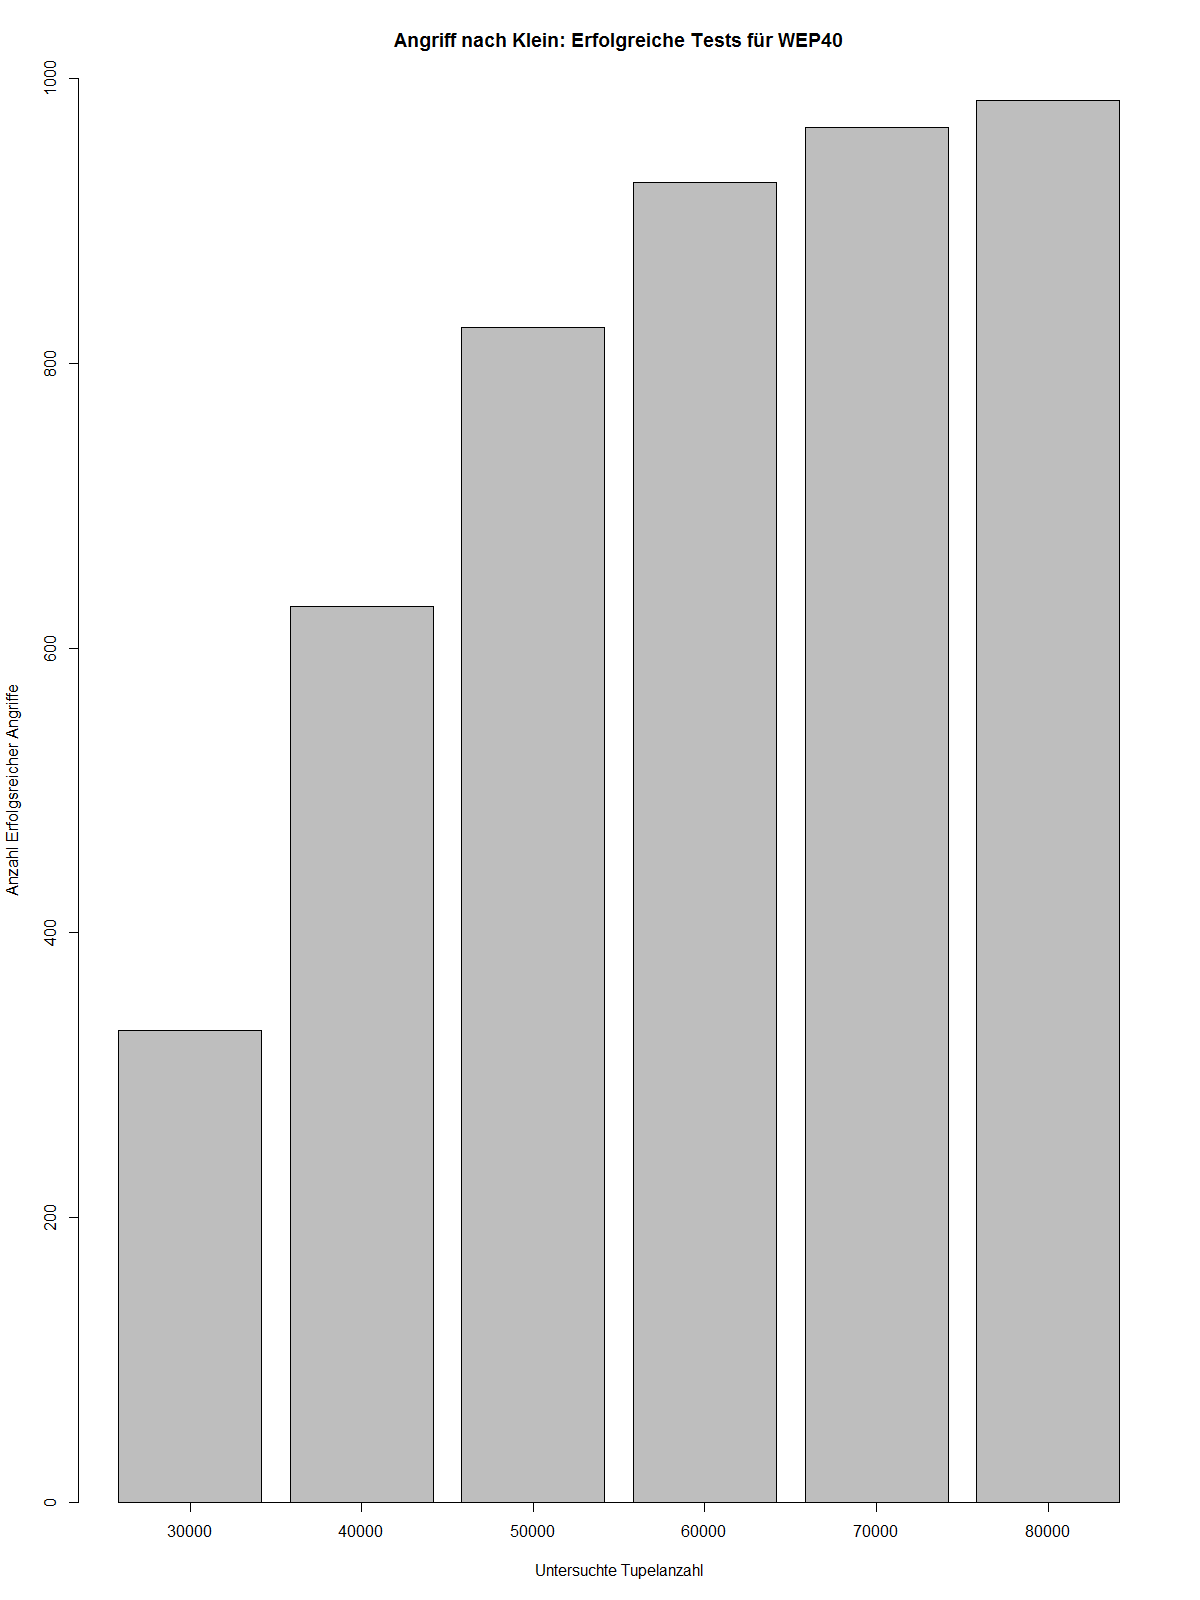
\includegraphics[width=0.9\textwidth]{img/wep40_erfolg.png}
\end{center}
\label{fig:wep40_suc}
\newpage

Die folgende Grafik zeigt ab wie vielen untersuchten Tupeln der verbesserte Angriff erfolgreich war. Hierfür wurden 3103 erfolgreiche Angriffe untersucht. 
\begin{center}
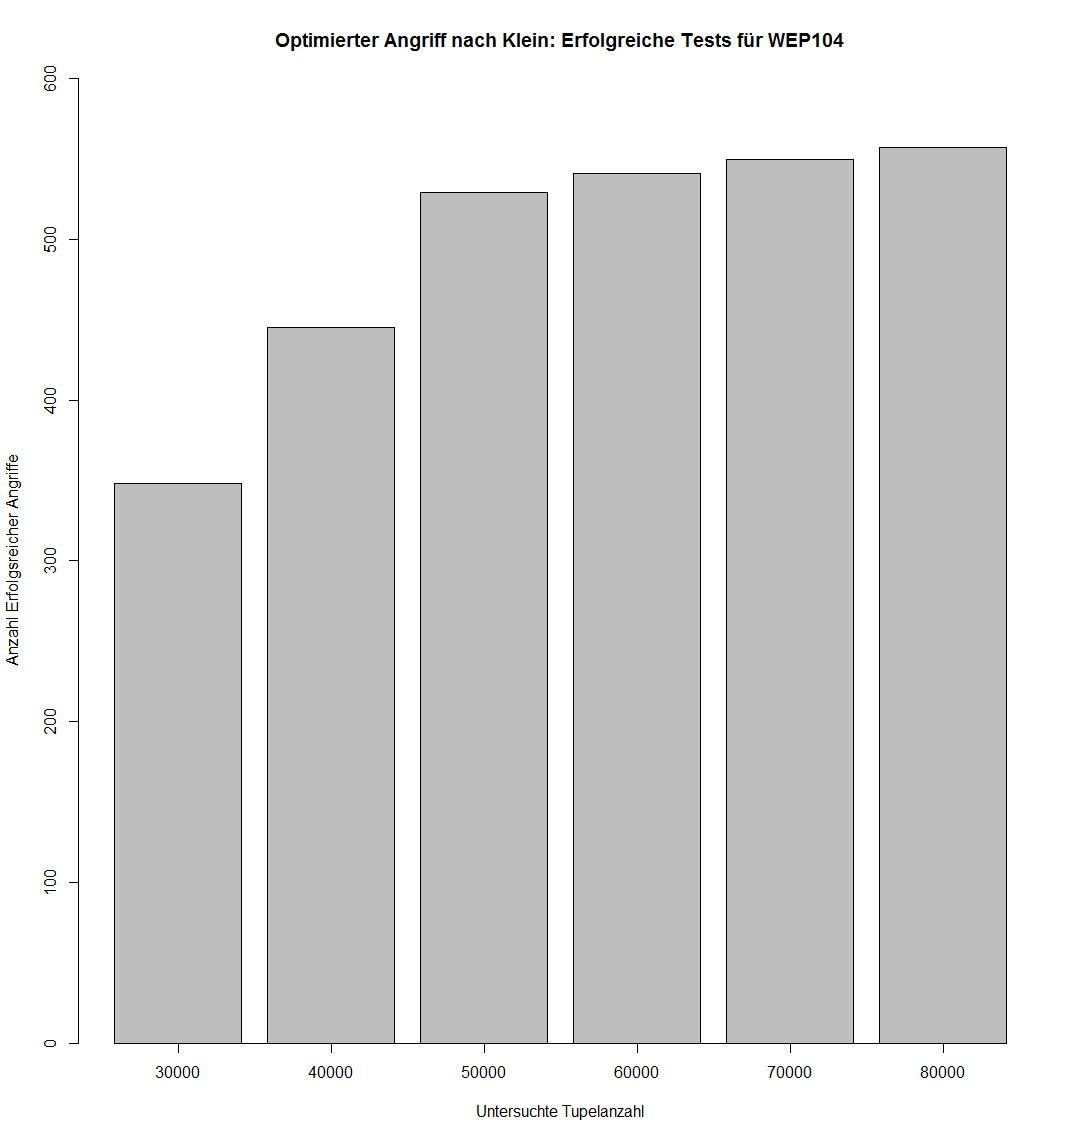
\includegraphics[width=0.9\textwidth]{img/WEP_104_erfolgreich.png}
\label{fig:wep100_suc}
\end{center}
\newpage

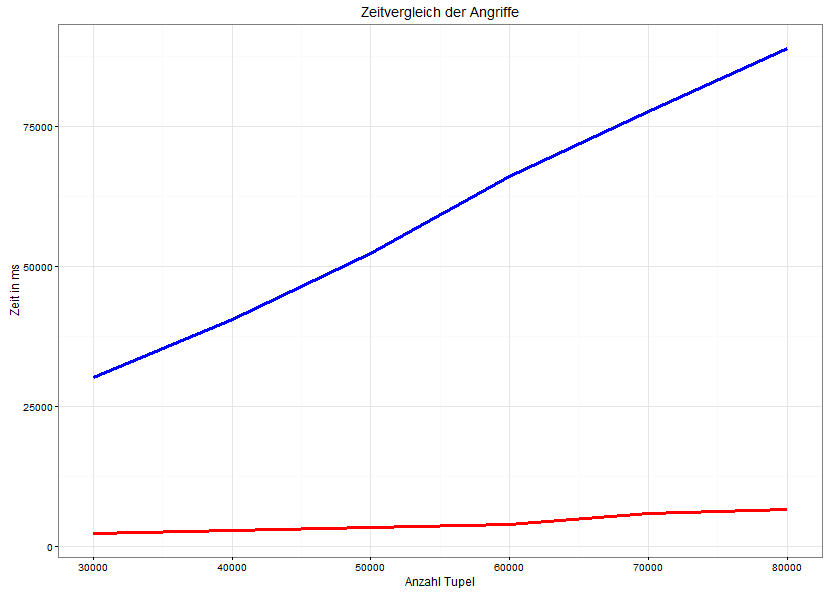
\includegraphics[width=\textwidth]{img/vergleich.png}
\label{fig:vergleich}
\\
\textbf{Legende}
\begin{itemize}
	\item[] Angriff von Klein in blau
	\item[] Verbesserter Angriff in rot
\end{itemize}


\newpage

\nocite{*}
\printbibliography
\end{document}
